\documentclass[varwidth=true, border=2pt]{standalone}
\usepackage{tikz}
\begin{document}

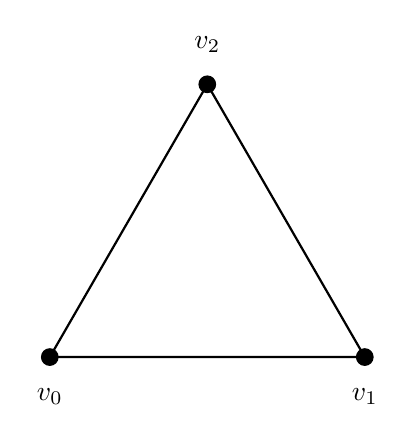
\begin{tikzpicture}
    \centering
    %% vertices
    \draw[fill=black] (0,0) circle (3pt);
    \draw[fill=black] (2,3.464) circle (3pt);
    \draw[fill=black] (4,0) circle (3pt);
    %% vertex labels
    \node at (0,-0.5) {$v_0$};
    \node at (4,-0.5) {$v_1$};
    \node at (2,3.964) {$v_2$};
    %\node at (6,-0.5) {3};
    %\node at (0, 0.5) {$\mathbb R$};
    %\node at (1, 0.5) {$\mathbb R$};
    %\node at (2, 0.5) {$\mathbb R$};
    %\node at (3, 0.5) {$\mathbb R$};   
    %\node at (4, 0.5) {0};
    %\node at (5, 0.5) {0};     
    %\node at (6, 0.5) {0};           
    %%% edges
    \draw[thick] (0,0) -- (4,0) -- (2,3.464) -- (0,0);
    %\caption{}
\end{tikzpicture}

\end{document}